\section{Preliminary results}
\label{sec:robots_results}
The DUA framework and the technologies presented so far have led to the development of a few prototypes during the time in which this thesis was drafted. These prototypes were developed either to perform specific tasks in real-world scenarios, or to test novel solutions in fields like robot autonomy and localization and mapping. The common ground of these prototypes is the use of the DUA framework in their development and deployment, which proved the effectiveness of the proposed solutions. This section presents some preliminary published results concerning the application of the technologies on which DUA is based to the field of autonomous robotics. Their success has brought to the formalization of the DUA framework as presented in \Cref{ch:dua}, as well as to the solutions presented in the previous \Cref{sec:dua-utils}.

\subsection{A \ROS distributed architecture for unmanned aircraft}
\label{sec:robots_results_paperdrone2021}
In \cite{bianchi_novel_2023}, a novel distributed architecture is designed and proposed for an autonomous drone, tasked with the execution of a target reconnaissance and precision landing mission in an indoor, GNSS-denied environment. The mission was part of the 2021 Edition of the Leonardo Drone Contest, a robotics competition hosted by Leonardo S.p.A. in which custom-built UASs have to perform a series of complex tasks autonomously, ranging from localization and flight control to environment mapping and autonomous navigation.

The research team from the Tor Vergata University of Rome participated in the 2021 Leonardo Drone Contest, which was conducted in Turin, Italy during September 2021. This competition featured six Italian universities deploying autonomous drones to execute a sophisticated mission within a structured indoor environment. The operational field was meticulously configured with various elements, including 10 distinct landing pads and 3 mobile ground robots, with all participants receiving comprehensive details about the field layout prior to the competition. The visual markers demarcating the landing pads provided additional navigational guidance. A depiction of the 2021 field layout is shown in \Cref{fig:ldc21field}: landing pads are in green and marked with their numerical ID, while known obstacles are in gray and their height in centimeters is reported.
\begin{figure}[t!]
  \centering
  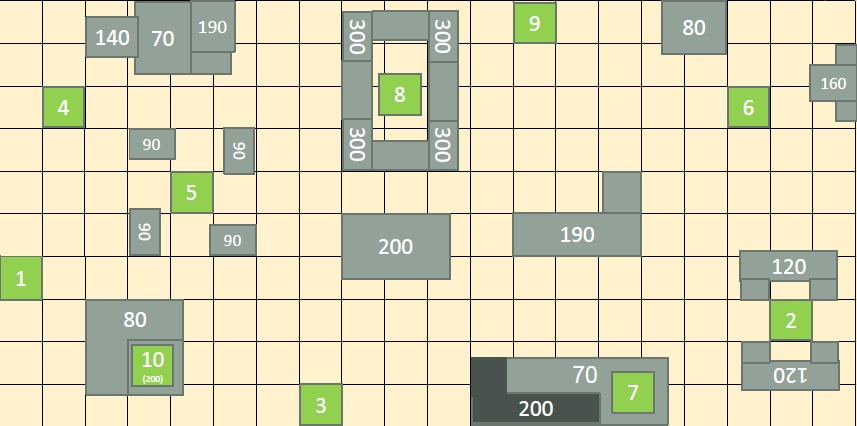
\includegraphics[width=.8\textwidth]{images/ch5/ldc21_field.jpg}
  \caption{The 2021 Leonardo Drone Contest field layout.}
  \label{fig:ldc21field}
\end{figure}

The mission objectives for each drone were structured as follows.
\begin{enumerate}
  \item Initiate take-off from a designated pad.
  \item Conduct environmental reconnaissance to locate one of the three ground-based mobile robots.
  \item Capture photographic documentation of the identified robot and transmit the imagery to an operator, who would subsequently communicate a specific landing sequence.
  \item Execute precision navigation between pads, performing sequential landings and take-offs according to the prescribed sequence.
\end{enumerate}

Participants were allowed to use a Ground Control Station (GCS) for mission initialization and continuous drone monitoring. The landing sequence was strategically determined by an operator at the GCS to optimize the cumulative score, which was calculated through the summation of points assigned to each successful landing on a given pad. The point distribution was uniquely encoded on the ground-based robot, so it required initial identification.

The competition imposed rigorous technical constraints on all participating teams. Specifically, the use of GNSS platforms was prohibited, and Light Detection and Ranging (LiDAR) sensors were expressly forbidden. Additionally, teams were precluded from deploying any fixed ground-based sensors or motion capture systems, thereby challenging participants to develop innovative autonomous navigation strategies using the few remaining sensors which were not only allowed, but also capable of being mounted on a small UAS.

To facilitate the comprehensive mission objectives, a sophisticated hardware and software architecture was meticulously designed and implemented on advanced hardware. The autonomous quadcopter developed for the Leonardo Drone Contest 2021 represents a complex system that not only meets the specified requirements but also serves as an optimal test framework for the methodologies introduced in \Cref{ch:tools}. The architectural design strategically partitions both hardware and software components across multiple hierarchical levels, addressing the distinct critical challenges inherent to each layer.

\subsubsection{Implementation details}
\label{sec:robots_results_paperdrone2021_impl}
The hardware architecture was composed by three distinct systems: a Holybro Pixhawk 4 flight controller (see \Cref{sec:dua_modules_flight_stack}), an Nvidia Jetson Xavier NX companion computer (see \Cref{sec:dua_supported_platforms_sbc}), and a PC acting as the Ground Control Station. The two embedded systems were mounted on the UAS prototype and interconnected as in \Cref{fig:ldc21hwarch}, which also depicts a functional diagram for the hardware architecture: the Pixhawk 4 flight controller is responsible for low-level flight control tasks, while the Nvidia Jetson Xavier NX companion computer executes high-level algorithms and mission-critical tasks and interfaces with the former to send commands and receive feedbacks and status data. A summary of the technical specifications of these two embedded systems is given in \Cref{tab:ldc21_sbcs}.
\begin{table}[t]
  \centering
  \begin{tabular}{|c|c|}
    \hline
    \multicolumn{2}{|c|}{\textbf{Nvidia Jetson Xavier NX}}\\
    \hline
    CPU & NVIDIA Carmel ARM v8.2 (6C/6T, up to \SI{1.4}{GHz})\\
    RAM & \SI{8}{GB} LPDDR4x\\
    GPU & NVIDIA Volta (384 CUDA Cores, 48 Tensor Cores)\\
    OS  & Ubuntu Linux 20.04\\
    \hline
    \multicolumn{2}{|c|}{\textbf{Holybro Pixhawk 4}}\\
    \hline
    CPU & STM32F765 (ARM Cortex-M7, up to \SI{216}{MHz})\\
    RAM & \SI{512}{KB}\\
    OS  & NuttX 10.0.0\\
    \hline
  \end{tabular}
  \caption{Main technical specifications of the SBCs used in the implementation.}
  \label{tab:ldc21_sbcs}
\end{table}

\Cref{fig:ldc21swarch} illustrates the comprehensive organization of software modules across functional layers.
\begin{itemize}
  \item \textbf{Lowest Layer:} Comprised of real-time modules critical for executing fundamental flight operations, as well as device drivers.
  \item \textbf{Middle Layers:} Hosts higher-level, computationally intensive algorithms responsible for executing individual mission tasks.
  \item \textbf{Highest Layer:} Dedicated to supervision logic, implemented as a Finite-State Machine (FSM), and the Ground Control Station (GCS) operator interface.
\end{itemize}
The architectural objective was to develop a cohesive set of \ROS modules that leverage interdependent functionality. This modular approach ensures vertical abstraction, enabling higher-level modules to operate without direct concern for lower-level implementation details such as take-off, landing, and navigational maneuvers. By abstracting these fundamental operations, the architecture promotes a clean, hierarchical system design that enhances modularity and operational flexibility.
\begin{figure}[t!]
  \centering
  \includesvg[width=\textwidth]{images/ch5/ldc21_swarch.svg}
  \caption{Software architecture of the LDC21 autonomous drone: thin arrows indicate communications established with \ROS interfaces, thick arrows represent dedicated software interfaces, white boxes represent \ROS nodes.}
  \label{fig:ldc21swarch}
\end{figure}

Regarding the set of software modules running on the UAS onboard computers, the lowest layer was composed of the early version of what has become the \texttt{flight\_stack} DUA unit presented in \Cref{sec:dua_modules_flight_stack}. This prototype was in fact running the very first version of this software, and it has provided a testbed for the development of a bridged DDS-based communication among the two levels of the onboard architecture.

The remaining layers contain modules that concern the following specific tasks: perception, navigation and exploration, and mission supervision. Regarding perception, the prototype was equipped with two Intel RealSense D435i depth cameras: one was pointed forward and used for localization, while the other was pointed downward and used for target detection. Both mobile robots and landing pads were equipped with ArUco markers \cite{romero-ramirez_speeded_2018,garrido-jurado_generation_2016}, a particular kind of fiducial markers with limited information aimed at improving detection probability and pose estimation capabilities. The \texttt{ArUco Scanner} module was responsible for detecting these markers and transmitting detection data to the \texttt{FSM} module, that ran a state machine to manage the mission phases and the drone behavior.

To understand the environment and get a consistent estimate of its position and orientation within it, the UAS ran a VSLAM (Visual Simultaneous Localization And Mapping) algorithm. The SLAM problem is notoriously complex and computationally intensive to solve, requiring sophisticated solutions from both the mathematical and implementation perspectives. Nonetheless, it was deemed as the only solution in this case due to the Contest rules: no sensors other than cameras were reliable enough to provide the required information, and due to accumulated error it was not possible to rely on odometry alone. The chosen VSLAM algorithm for this implementation was the ORB-SLAM2 system \cite{mur-artal_orb-slam2_2017}, a state-of-the-art solution for monocular, stereo, and RGB-D cameras that provides real-time performance and high accuracy in both localization and mapping tasks.

The \texttt{VSLAM} module was responsible for running the algorithm and providing the estimated pose of the drone directly to the PX4 firmware. The ORB-SLAM2 system employs binary feature extraction from input frames to construct a local map while addressing bundle adjustment optimization problems. To maximize computational efficiency and optimize memory utilization, these features are consistently employed throughout the entire system. The algorithm designates certain frames as keyframes, which serve as critical reference points for the local map structure. These keyframes are instrumental in computing the current local pose through the construction of a \emph{covisibility graph}, which facilitates both localization and environmental mapping functions. As the map increases in scale, the system generates an additional structural representation known as the \emph{essential graph}, which enables loop detection capabilities. Upon loop detection, the system executes an automatic loop closure procedure wherein all graphs undergo analysis and updating. During this process, redundant keyframes and nodes are eliminated, and the local map undergoes revision incorporating recent measurements to minimize systematic errors.

The architecture of the ORB-SLAM2 system comprises four distinct operational phases: tracking, local mapping, loop closing, and global adjustment. Each phase executes in a dedicated thread. The tracking phase monitors scene features, while local mapping utilizes these same features to construct the local map in relation to the established keyframes. The loop closing phase identifies potential loops and communicates this information to the global adjustment thread, which performs global bundle adjustment across the entire map to enhance overall accuracy.

ORB-SLAM2 supports multiple input modes: monocular, stereo, and RGB-D. The implementation used in this work introduces an additional mode that uses infrared and depth images, called IRD mode. This modification addresses specific technical limitations of Intel RealSense cameras, particularly the temporal misalignment between RGB and depth frames, while maintaining proper synchronization with infrared frames. Significant modifications to the ORB-SLAM2 algorithm have been implemented to expand parameter control capabilities, incorporate ARM processor compatibility, and integrate NVIDIA CUDA GPU optimizations. The adaptation for ARM architecture required the disabling of x86-specific optimizations, particularly affecting performance in feature extraction and computation phases that previously leveraged AVX/SSE vector instruction sets. To address these performance implications, CUDA GPU optimization became essential. Within the distributed architecture shown in \Cref{fig:ldc21swarch}, this algorithm operates as a \ROS node, consuming camera topic frames and publishing both the current pose estimation and system state on separate topics.

The next task to address was that of autonomous navigation and exploration of the environment, to find ground targets and landing zones. The \texttt{Navigator} module was implemented for this purpose, with the aim of providing a high-level interface to navigation operations. These operations were exposed as \ROS synchronous communication primitives, \emph{i.e.}, in the form of services: their refinement as more complex operations requiring a stateful communication was left as future work and developed for subsequent prototypes. The \texttt{Navigator} module was responsible for sending commands to the lower levels to move the drone from its current position to a given target position, provided that such a position was reachable and that there existed a path to reach it. This additional task of computing and returning paths was left to the \texttt{Path Finder} module: its primary objective was to determine an optimal trajectory between current and target positions that simultaneously minimizes distance while ensuring collision avoidance. The implemented solution approaches path planning through graph construction representing traversable space within the environment. Trajectory optimization utilizes the A* search algorithm \cite{guruji_time-efficient_2016}.

The algorithm initially constructs a graph representation directly from environmental point cloud data acquired via ORB-SLAM2. This process begins by discretizing the environment into a three-dimensional grid of variable-resolution cubic cells, each identified by its centroid. The interconnection network of traversable cells constitutes the graph structure. Boundary cells are automatically designated as non-traversable to constrain the UAS operational space. Environmental obstacle identification proceeds through point cloud preprocessing, beginning with the removal of out-of-bounds points. The algorithm associates points with their containing cells, designating cells exceeding a predetermined point density threshold as non-traversable. The remaining cells form the graph vertex set, followed by edge construction. For each cell, the algorithm identifies neighboring cells in eight coplanar directions at equal altitude, plus immediate vertical neighbors. Edge insertion between adjacent cells depends on a corridor analysis based on the physical dimensions of the drone: an edge is established if and only if the point density within the corridor falls below a specified threshold. This methodology enables variable-resolution environmental discretization while maintaining consideration for the physical footprint of the drone during transitions.

Valid corridors result in edge insertion with costs equal to the Euclidean distance between cell centroids. This iterative process yields a graph representation of the operational space, computed offline. The designated \texttt{Path Finder} \ROS node implements a computationally optimized A* algorithm to determine shortest paths between arbitrary nodes upon request, carried over a service interface. Path finding operations begin with origin and target cube identification and validation. Upon confirming traversability, the algorithm initiates shortest path computation, returning a sequence of waypoints leading to the target position. The selection of A* is motivated by its mathematical properties of admissibility, completeness, and optimality. As an informed search algorithm, A* leverages domain knowledge through heuristic guidance, distinguishing it from other similar algorithms. In the context of three-dimensional navigation, the implementation employs Euclidean distance as its heuristic function, facilitating efficient minimum-distance path identification.

\subsubsection{Supervision}
\label{sec:robots_results_paperdrone2021_supervision}
The software architecture culminates in a finite-state machine that implements high-level supervision logic. This FSM presents the drone as an automaton executing complete missions within the Leonardo Drone Contest parameters while managing contingencies such as hardware failures, battery depletion, and localization system degradation or complete failure. State transitions trigger formulation of requests to subordinate modules, with transitions conditioned upon both current state and intervening events.

The implementation integrates with the distributed architecture through a \ROS node that facilitates bidirectional communication with other modules via service calls and alert reception. System initialization comprises a comprehensive status verification of all modules through \ROS middleware APIs; mission execution begins only upon confirmation of full operational readiness across all subsystems.

The structure of the FSM mirrors mission dynamics as specified in the Contest rules. The implementation consolidates all abstraction levels into a single routine where state transitions are invoked based on the operational conditions of the drone following each execution step. Error handling leverages the meta-machine concept: primary mission phases execute within states comprising a subordinate FSM, while maintaining guaranteed transition paths to termination states under all circumstances. The high-level and low-level FSMs are shown in \Cref{fig:ldc21fsmhl,fig:ldc21fsmll}.
\begin{figure}[t!]
  \centering
  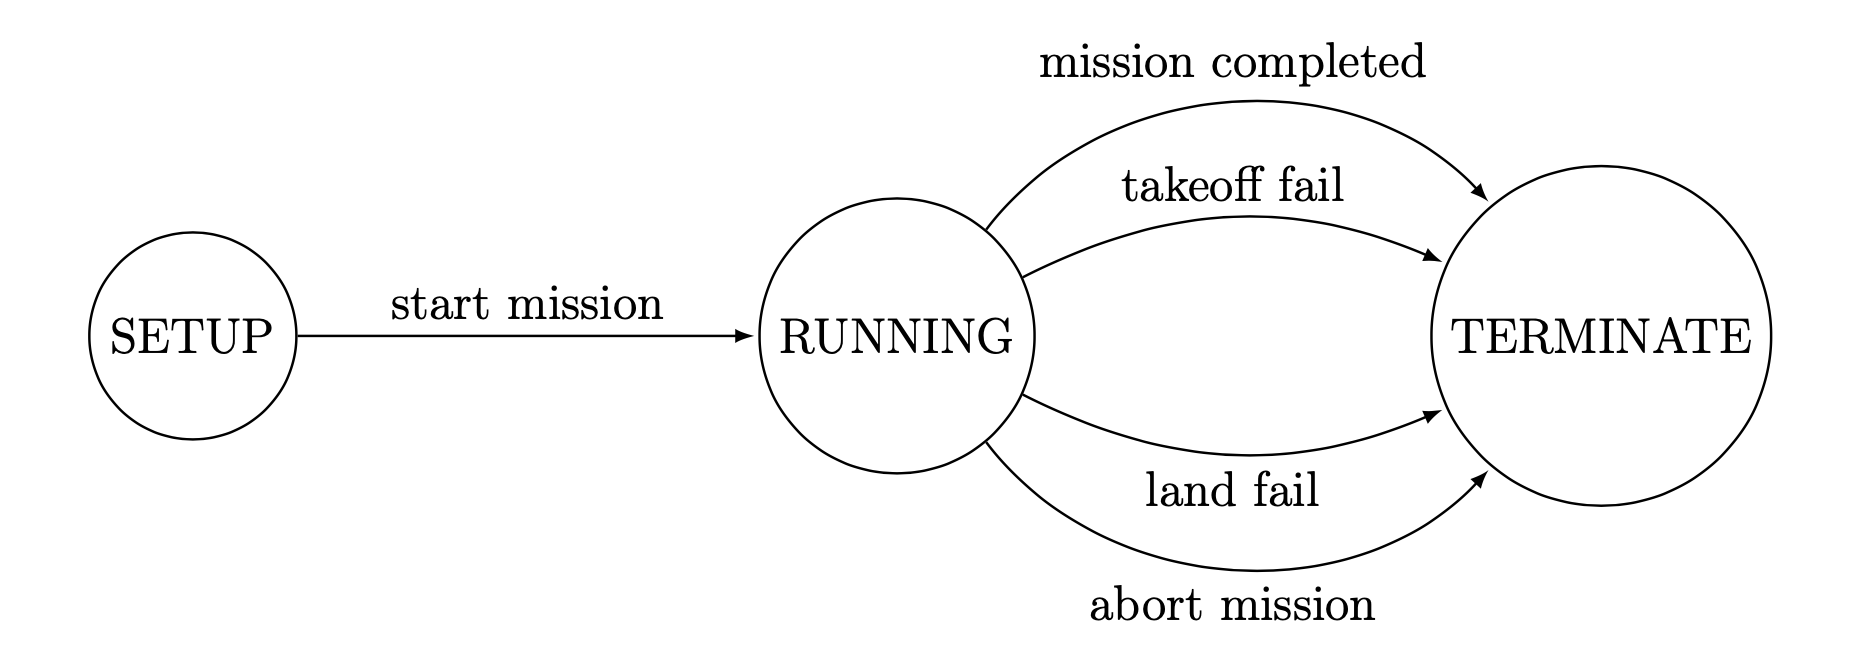
\includegraphics[width=.9\textwidth]{images/ch5/ldc21_FSM_HL.png}
  \caption{High-level finite-state machine for the Leonardo Drone Contest 2021 mission.}
  \label{fig:ldc21fsmhl}
\end{figure}
\begin{figure}[t!]
  \centering
  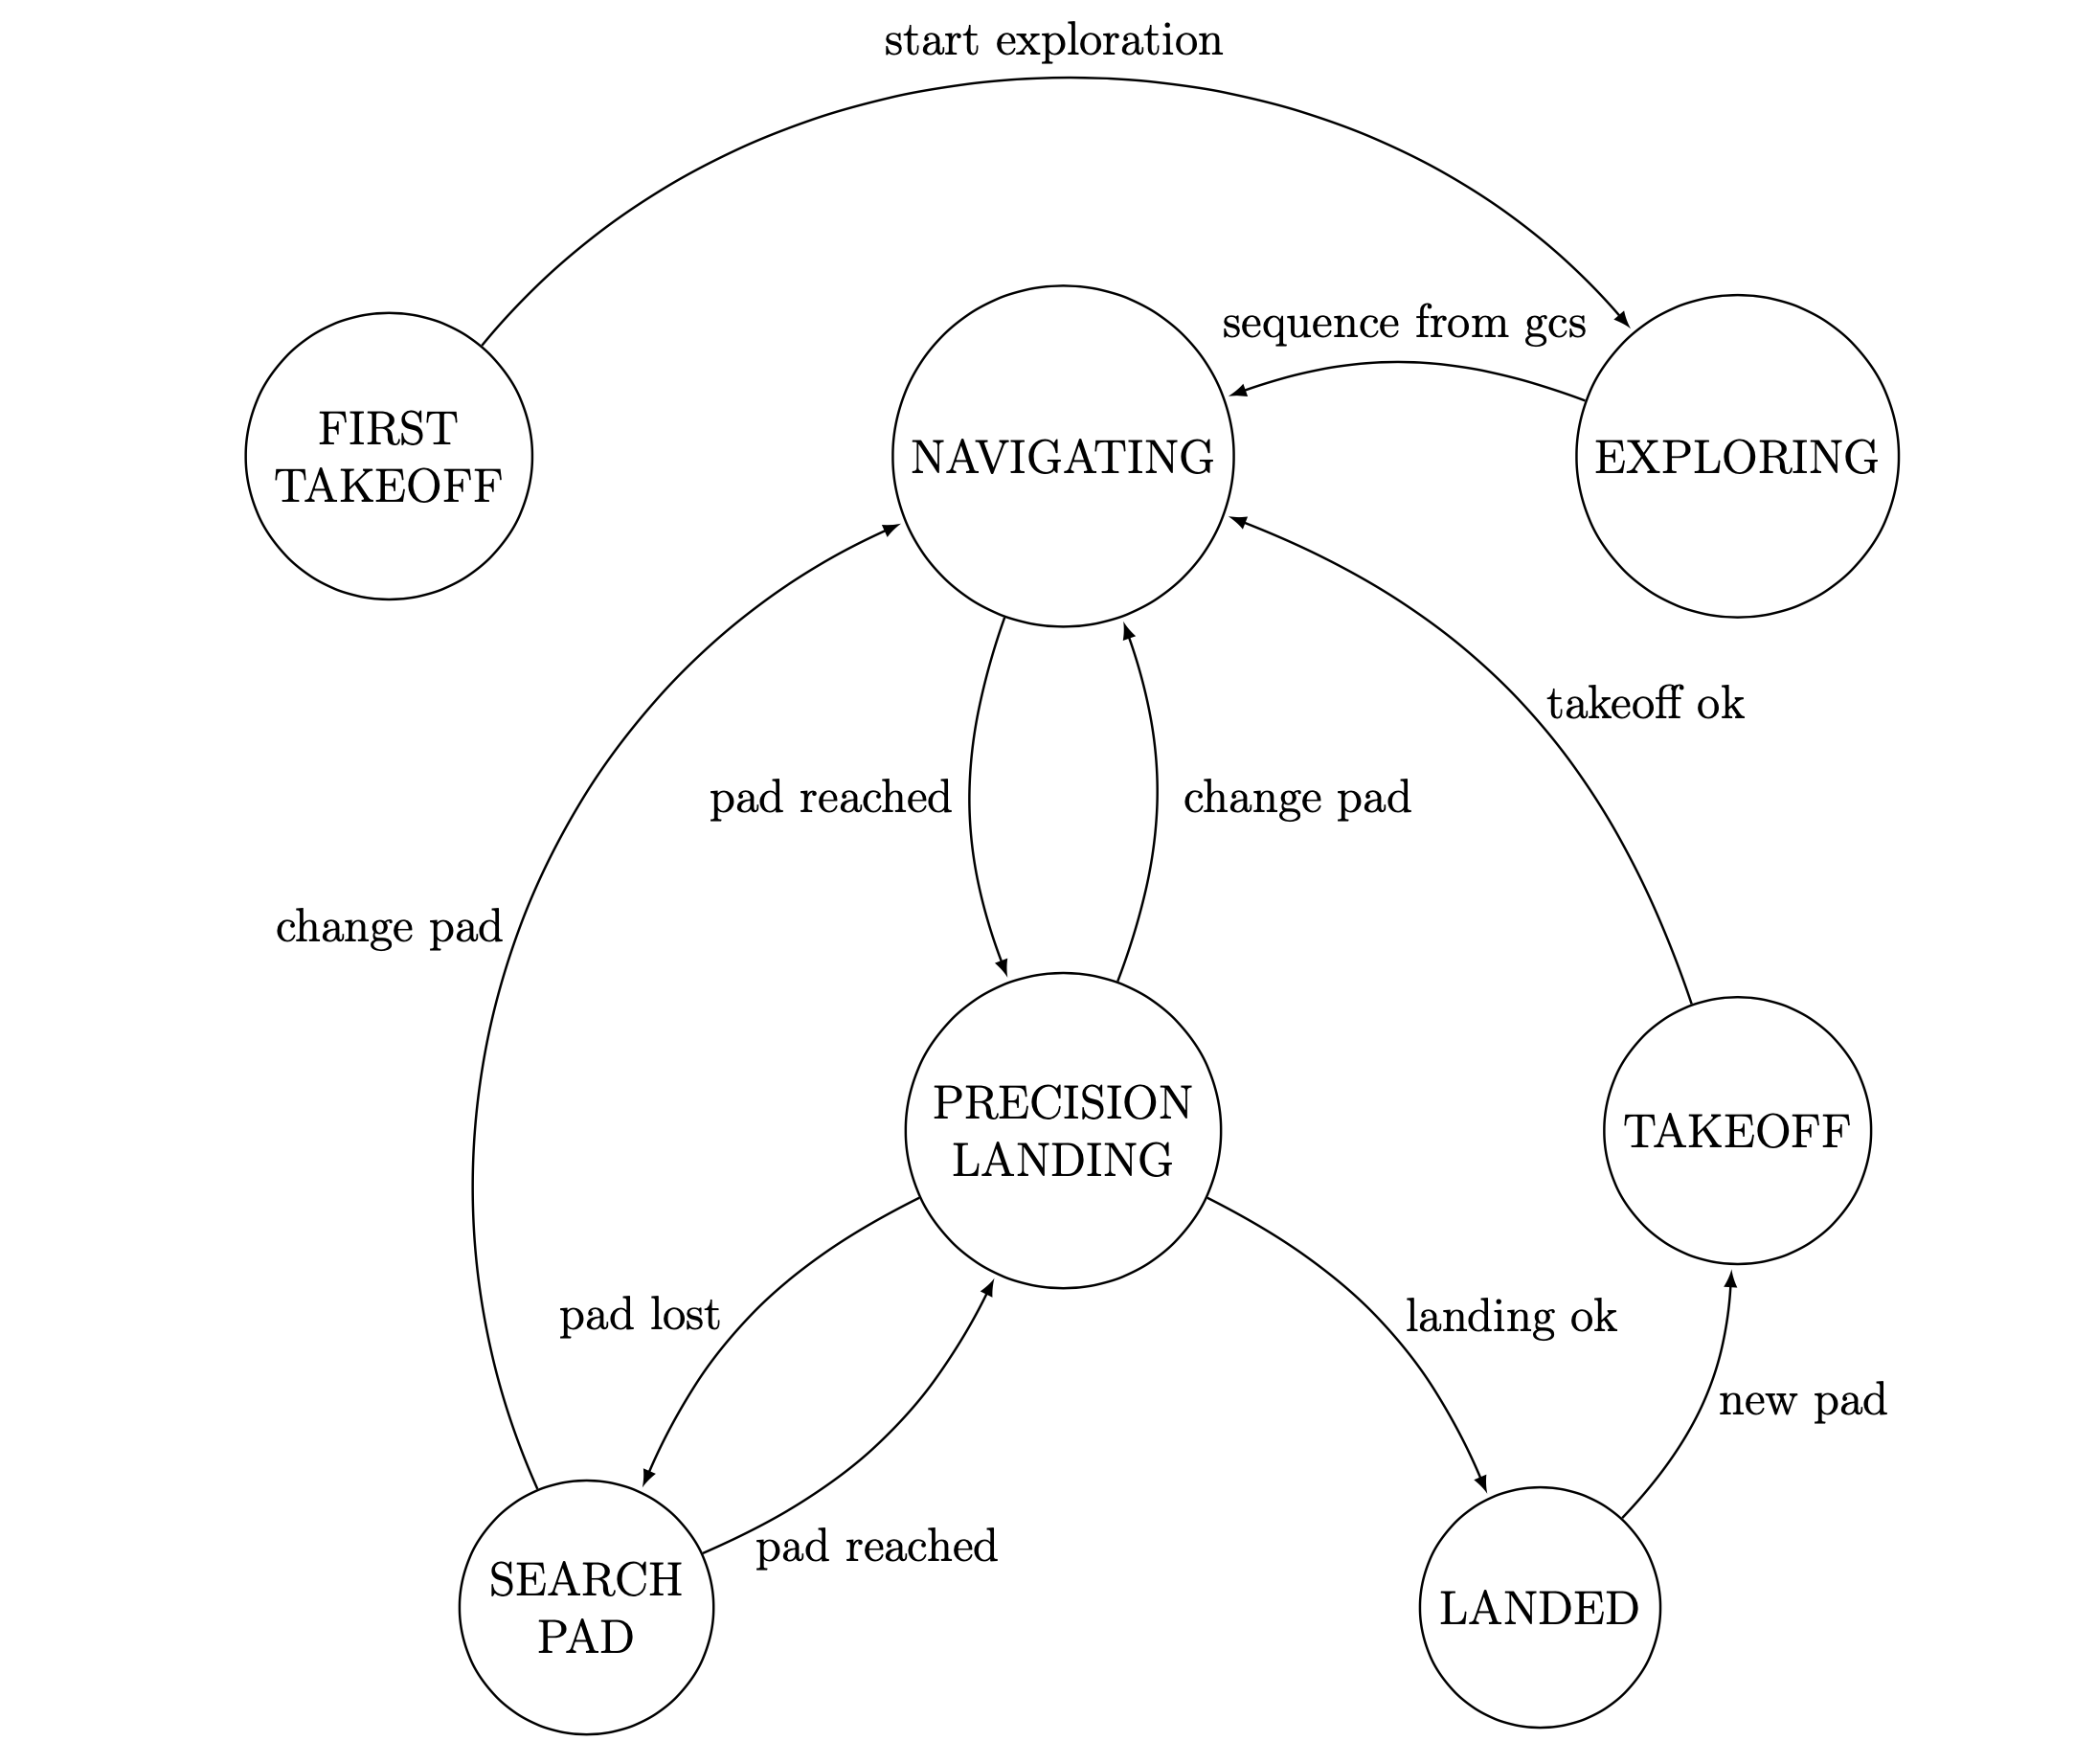
\includegraphics[width=.9\textwidth]{images/ch5/ldc21_FSM_LL.png}
  \caption{Low-level finite-state machine for the Leonardo Drone Contest 2021 mission.}
  \label{fig:ldc21fsmll}
\end{figure}

\subsubsection{Experimental results}
\label{sec:robots_results_paperdrone2021_results}

\begin{figure}[t!]
	\centering
	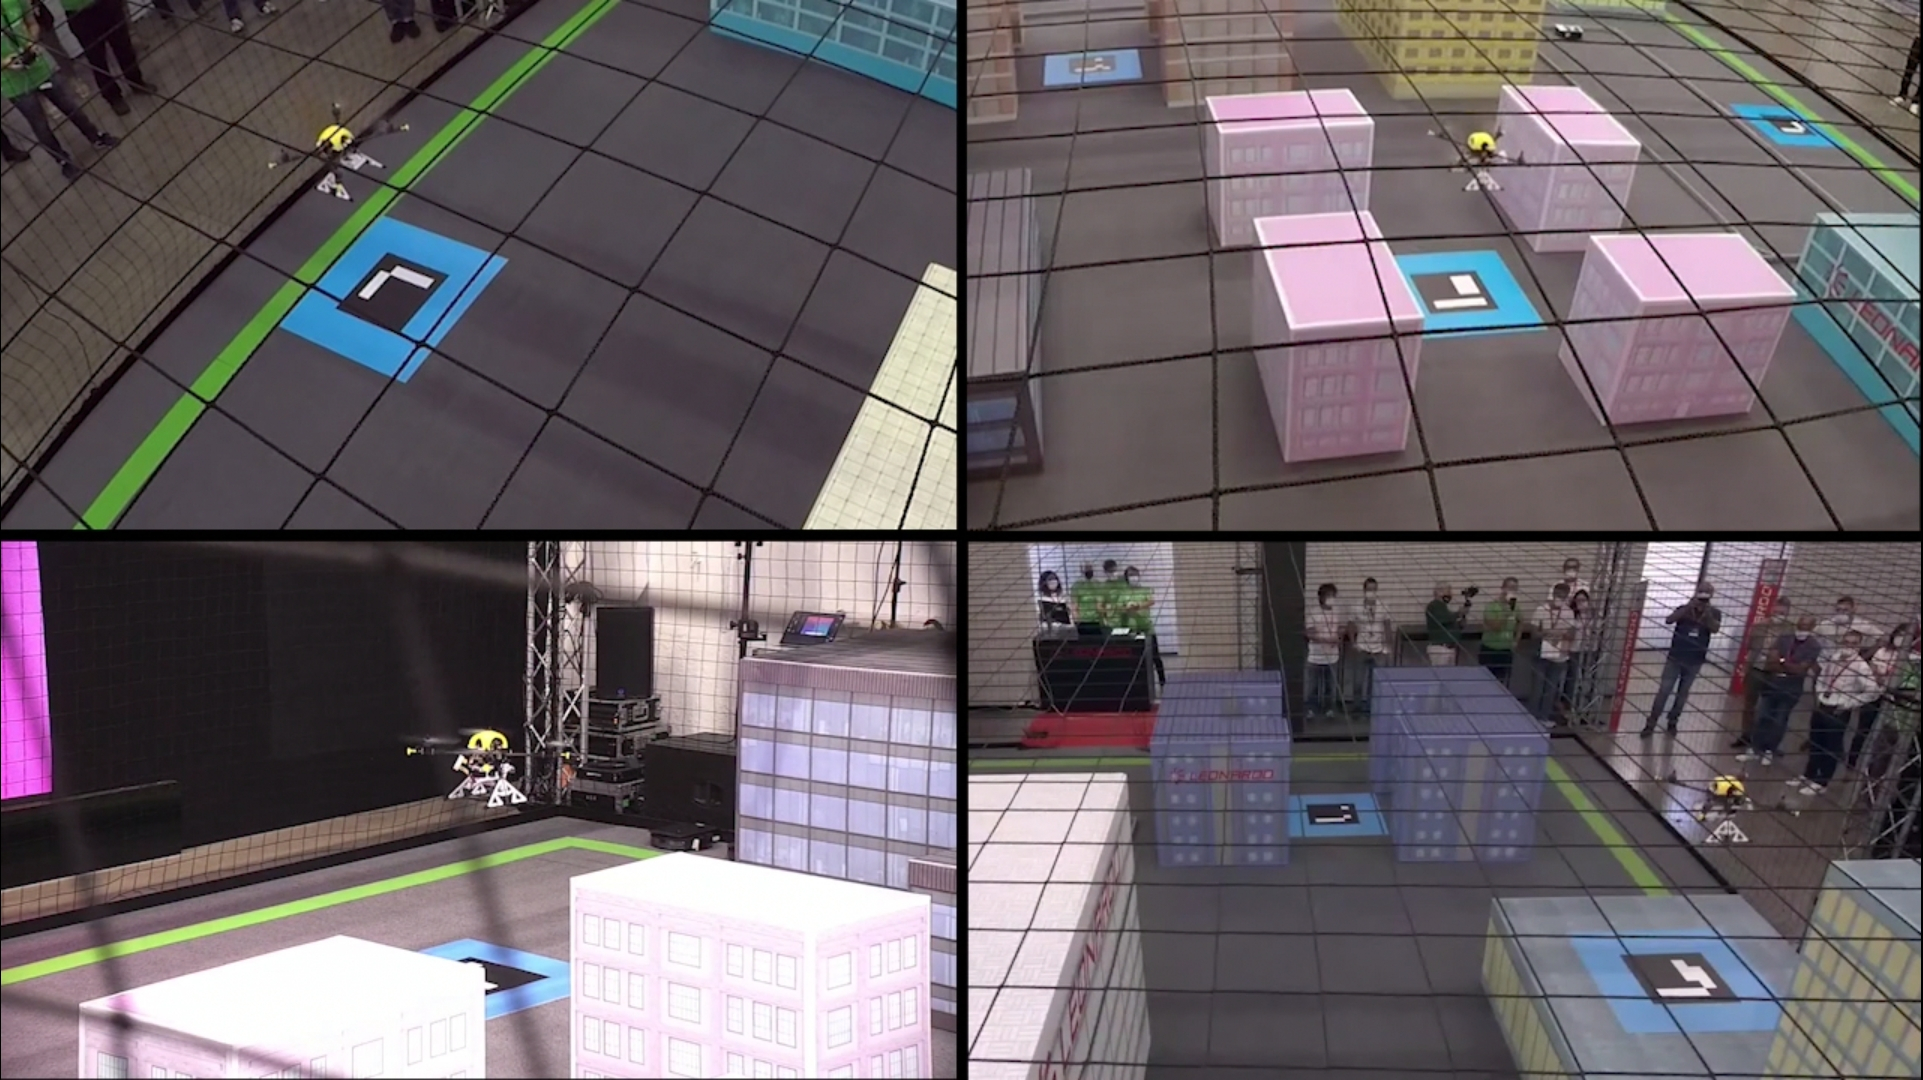
\includegraphics[width=.9\textwidth]{images/ch5/ldc21_frame1.jpg} \\
	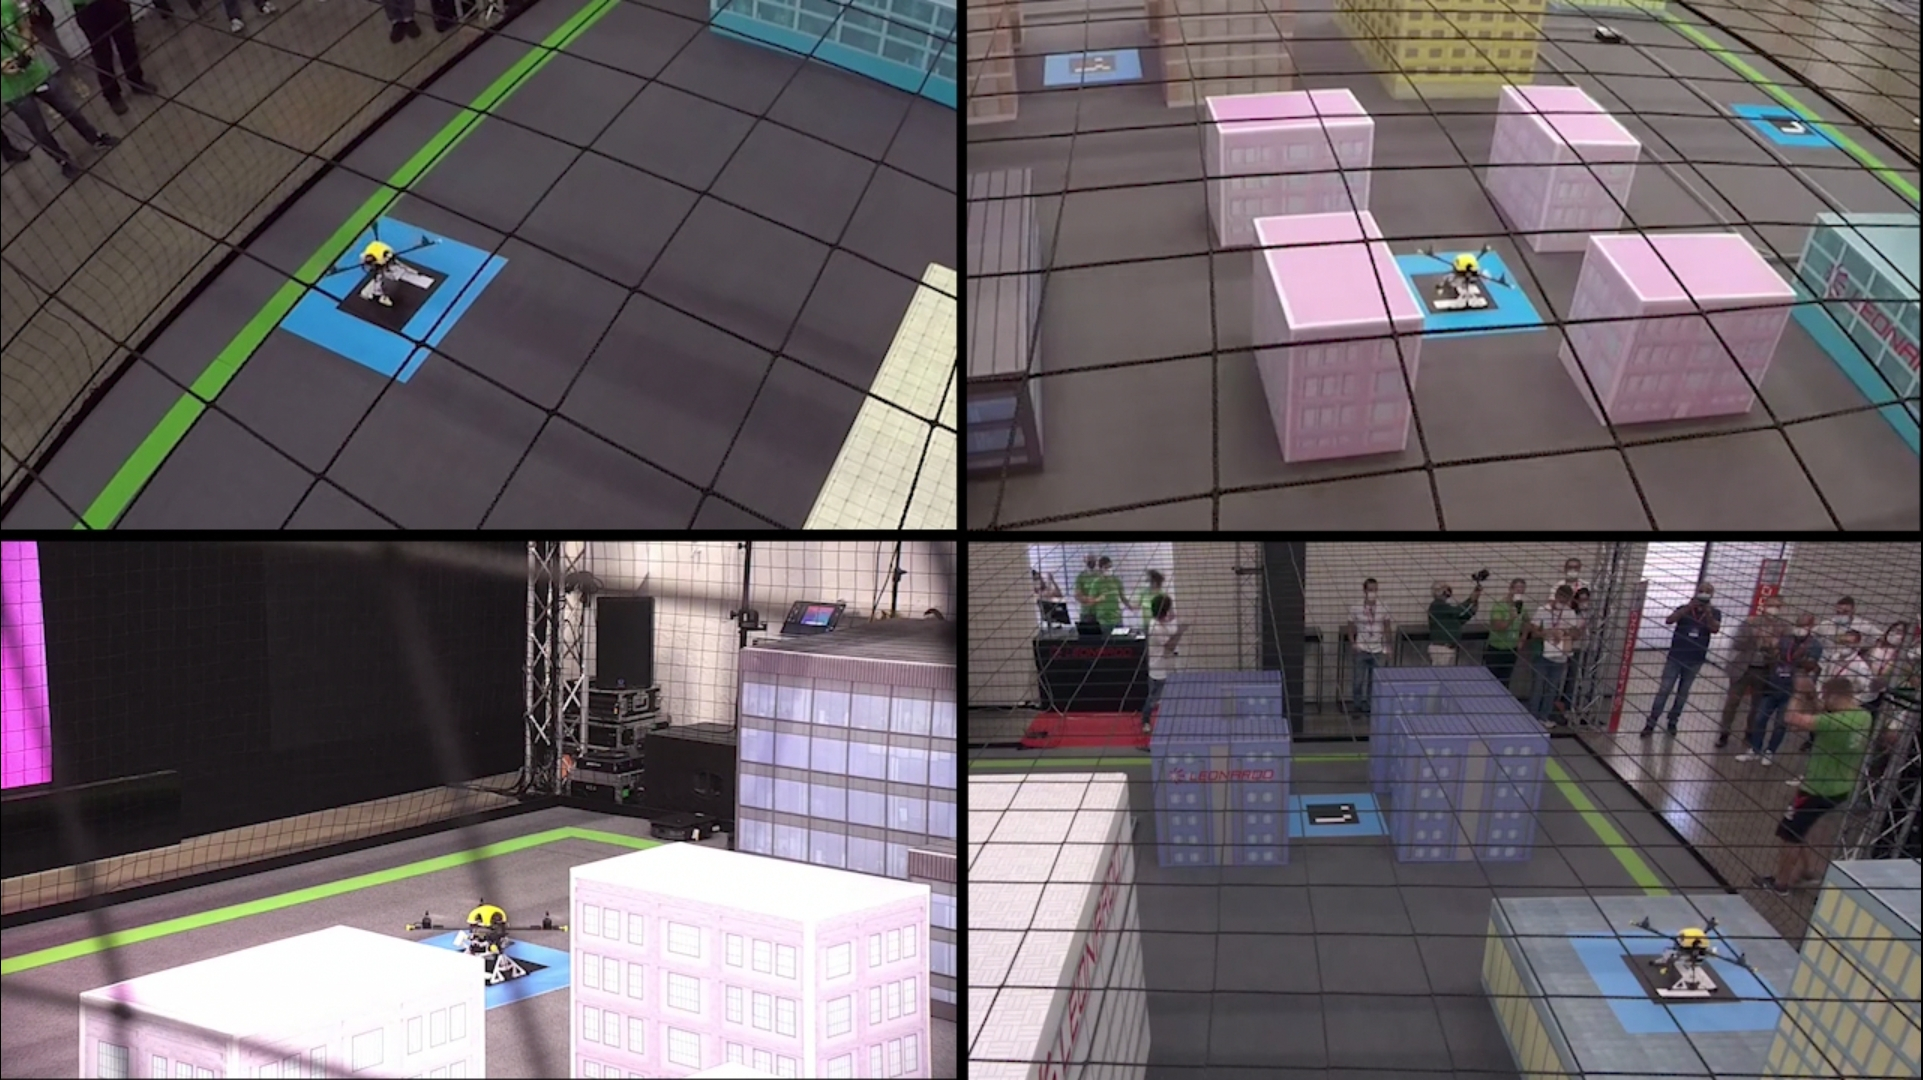
\includegraphics[width=.9\textwidth]{images/ch5/ldc21_frame2.jpg}
	\caption{Successful precision landings performed on the ArUco landing pads during the 2021 Leonardo Drone Contest.}
	\label{fig:ldc21_preclands}
\end{figure}
